% --------------------------------------------------------------------------------

\begin{exercise}

Lösen Sie folgendes Problem für $x > 0$ mithilfe der Methode der Charakteristiken:

\begin{align*}
    -y u_x + x u_y
    & =
    u + 1 \\
    u(x, 0)
    & =
    \psi(x)
\end{align*}

wobei $\psi$ eine beliebige Funktion ist.

\end{exercise}

% --------------------------------------------------------------------------------

\begin{solution}

Wir bringen zunächst die PDE in die allgemeine Form aus dem Skript (bzw. Vorlesung).

\begin{gather*}
    a(x, y, u) = -y,
    \quad
    b(x, y, u) = x,
    \quad
    c(x, y, u) = u + 1, \\
    \overline{x}(t) = t,
    \quad
    \overline{y}(t) = 0,
    \quad
    \overline{u}(t) = \psi(t), \\
    \Gamma = \Bbraces
    {
        (
            (
                \overline{x}(t),
                \overline{y}(t)
            ):
            t \in \R
        )
    } \in \R^2,
    \quad
    S = \Bbraces
    {
        (
            (
                \overline{x}(t),
                \overline{y}(t),
                \overline{u}(t)
            ):
            t \in \R
        )
    } \in \R^3
\end{gather*}

Die folgende Abbildung \ref{fig:MdCS} soll die räumliche Intuition hinter der Methode der Charakteristiken wiederholen.

\begin{figure}[h!]
    \centering
    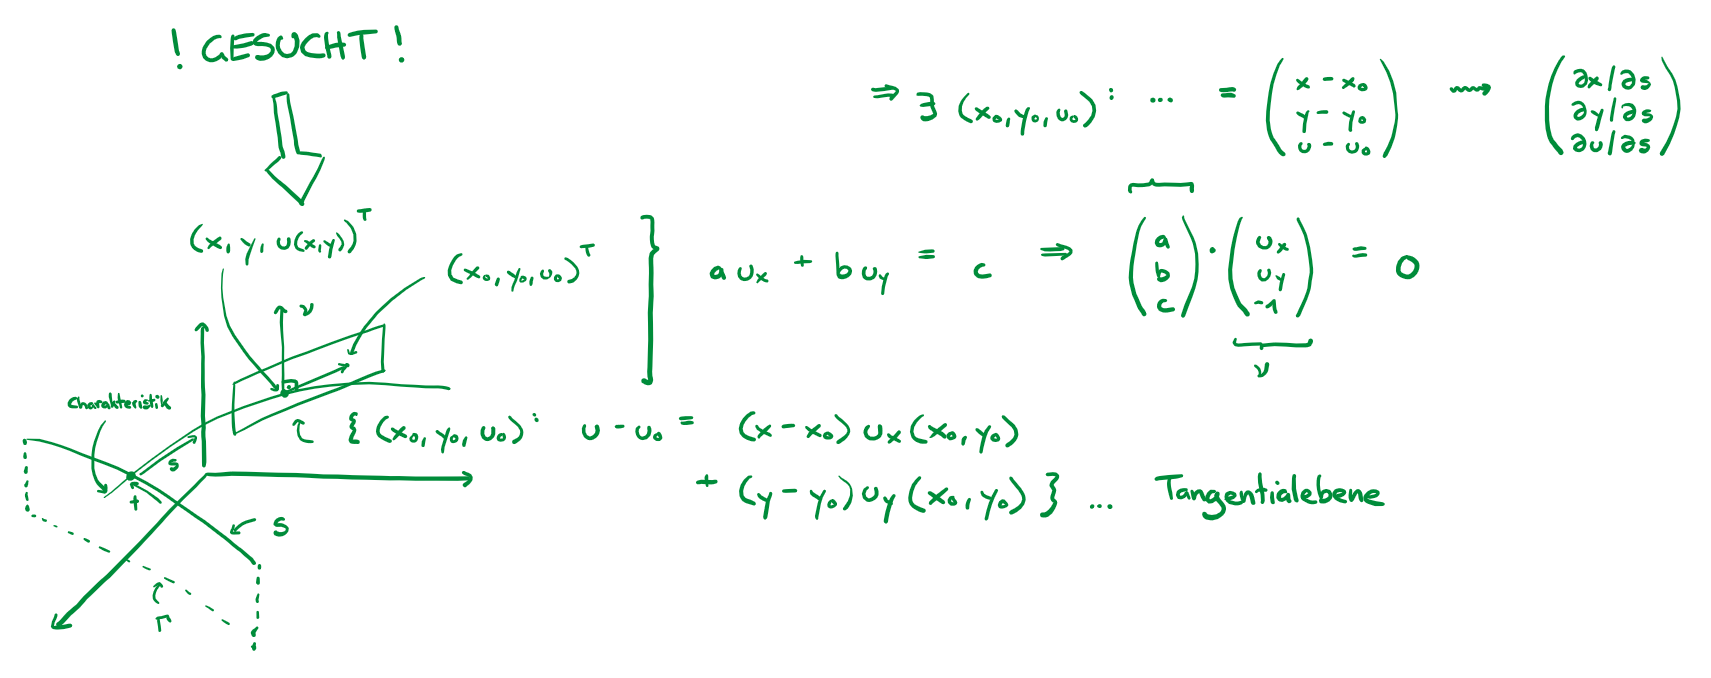
\includegraphics[width = \textwidth]{Methode der Charakteristiken - Skizze.png}
    \caption{Methode der Charakteristiken - Skizze}
    \label{fig:MdCS}
\end{figure}

Das dazugehorige Anfangswertproblem lautet

\begin{align*}
    \pderivative[][x]{s} = a = -y,
    \pderivative[][y]{s} = b = -x,
    \pderivative[][u]{s} = c = u + 1,
\end{align*}

mit Anfangswerten

\begin{align*}
    x(0, t) = \overline{x}(t) = t,
    y(0, t) = \overline{y}(t) = 0,
    u(0, t) = \overline{u}(t) = \psi(t).
\end{align*}

Wir lösen die ODE für festes $t$ als folgendes inhomogene lineare System mit konstanten koeffizienten.

\begin{align*}
    v(s)
    :=
    \begin{pmatrix}
        x(s, t) \\ y(s, t) \\ u(s, t)
    \end{pmatrix}
    \implies
    v^\prime
    =
    \underbrace
    {
        \begin{pmatrix}
             0 & 1 & 0 \\
            -1 & 0 & 0 \\
             0 & 0 & 1
        \end{pmatrix}
    }_{=: A} v
    +
    \underbrace
    {
        \begin{pmatrix}
            0 \\ 0 \\ 1
        \end{pmatrix}
    }_{=: b},
    \quad
    v(0)
    =
    \begin{pmatrix}
        t \\ 0 \\ \psi(t)
    \end{pmatrix}
\end{align*}

Um die partielle Lösung $v$ zu bekommen, brauchen wir zuerst eine (alle) homogene(n).
Damit, ist ein Fundamentalsystem gemeint.
Nachdem die ODE konstante Koeffizienten hat, ist die Exponentialmatrix $e^{sA}$ ein Solches.
Um sie zu finden, müssen wir $A$ diagonalisieren (oder zumindest die Jordan-Normalform finden).
Dazu, berechnen wir die Eigenwerte $\lambda_{1, 2, 3}$ von $A$, als Nullstellen des Charakteristischen Polynoms $\chi_A$.
Man  kann  sich,  durch  Laplace-entwickelnnach der rechten (unteren) Spalte (Zeile) viel Arbeit ersparen.

\begin{align*}
    & \implies
    \chi_A(\lambda)
    =
    \begin{vmatrix}
        -\lambda &  1       & 0 \\
        -1       & -\lambda & 0 \\
         0       &  0       & 1 - \lambda
    \end{vmatrix}
    =
    (1 - \lambda)
    \begin{vmatrix}
        -\lambda & 1 \\
        -1       & -\lambda
    \end{vmatrix}
    =
    (1 - \lambda) (1 + \lambda^2)
    =
    (1 - \lambda) (1 - i) (1 + i) \\
    & \implies
    \lambda_{1, 2, 3} = 1, \pm i
\end{align*}

Die Eigenvektoren $v_{1, 2, 3}$ von $A$ dürfen auch nicht fehlen.
Das verläuft nach folgendem Schema $\Forall i = 1, 2, 3:$

\begin{align*}
    A v_i = \lambda_i v_i
    \iff
    (A - \lambda_i) v_i = 0
    \iff
    v_i \in \ker{(A - \lambda_i)}
\end{align*}

Konkret ...

\begin{align*}
    A - \lambda_1
    \mapsto &
    \begin{pmatrix}
        -1 &  1 & 0 \\
        -1 & -1 & 0 \\
         0 &  0 & 0
    \end{pmatrix}
    \mapsto
    \begin{pmatrix}
        -2 &  0 & 0 \\
        -1 & -1 & 0 \\
         0 &  0 & 0
    \end{pmatrix}
    \mapsto \cdots \mapsto
    \begin{pmatrix}
        1 & 0 & 0 \\
        0 & 1 & 0 \\
        0 & 0 & 0
    \end{pmatrix}
    \implies
    v_1
    \in
    \Span \Bbraces
    {
        \begin{pmatrix}
            0 \\ 0 \\ 1
        \end{pmatrix}
    } \\
    A - \lambda_2
    \mapsto &
    \begin{pmatrix}
        -i &  1 & 0 \\
        -1 & -i & 0 \\
         0 &  0 & 1 - i
    \end{pmatrix}
    \mapsto
    \begin{pmatrix}
         1 &  i & 0 \\
        -1 & -i & 0 \\
         0 &  0 & 1 - i
    \end{pmatrix}
    \mapsto \cdots \mapsto
    \begin{pmatrix}
        1 & i & 0 \\
        0 & 0 & 0 \\
        0 & 0 & 1
    \end{pmatrix}
    \implies
    v_2
    \in
    \Span \Bbraces
    {
        \begin{pmatrix}
            -i \\ 1 \\ 0
        \end{pmatrix}
    } \\
    A - \lambda_3
    \mapsto &
    \begin{pmatrix}
         i & 1 & 0 \\
        -1 & i & 0 \\
         0 & 0 & 1 + i
    \end{pmatrix}
    \mapsto
    \begin{pmatrix}
         1 & -i & 0 \\
        -1 &  i & 0 \\
         0 &  0 & 1 + i
    \end{pmatrix}
    \mapsto \cdots \mapsto
    \begin{pmatrix}
        1 & -i & 0 \\
        0 &  0 & 0 \\
        0 &  0 & 1
    \end{pmatrix}
    \implies
    v_3
    \in
    \Span \Bbraces
    {
        \begin{pmatrix}
            i \\ 1 \\ 0
        \end{pmatrix}
    }
\end{align*}

Die Eigenpaare (samt algebraischen Vielfachheiten) bekommt man auch ganz leicht mit \verb|SymPy|.

\begin{lstlisting}

A = sp.Matrix([[0, 1, 0], [-1, 0, 0], [0, 0, 1]])
display(A)

eigen_info = A.eigenvects()
display(eigen_info)

\end{lstlisting}

Wir fassen die Eigenvektoren (jeweils die angegebenen Repräsentanten) in eine Transformationsmatrix $V := (v_1, v_2, v_3)$ zusammen, und und berechnen deren Determinante.
Man kann sich, durch Laplace-entwickeln nach der linken (unteren) Spalte (Zeile) viel Arbeit ersparen.

\begin{align*}
    \implies
    \det{V}
    =
    \begin{vmatrix}
        0 & -i & i \\
        0 &  1 & 1 \\
        1 &  0 & 0
    \end{vmatrix}
    =
    (-1)
    \begin{vmatrix}
        -i & i \\
         1 & 1
    \end{vmatrix}
    =
    (-1) (-i - i)
    =
    2i \neq 0
\end{align*}

Nachdem die Determinante $\det{V}$ nicht verschwindet, muss $V$ invertierbar sein.
Wir invertieren $V$ wie üblich:
Durch Spaltenumformungen (d.h. von links drauf-multiplizieren von geeigneten regulären Permutations-Matrizen $P_1, \ldots, P_n$), so lange, bis

\begin{align*}
    P V = I_3
    \iff
    P I_3 = V^{-1},
    \quad
    P := \prod_{i=1}^n P_i.
\end{align*}

Der Übersicht halber, schreiben wir die Matrizen über bzw. unter einander.

\begin{multline*}
    \implies
    \begin{bmatrix}
        V \\
        \hline
        I_3
    \end{bmatrix}
    =
    \begin{bmatrix}
        0 & -i & i \\
        0 &  1 & 1 \\
        1 &  0 & 0 \\
        \hline
        1 & 0 & 0 \\
        0 & 1 & 0 \\
        0 & 0 & 1
    \end{bmatrix}
    \stackrel{P_1}{\mapsto}
    \begin{bmatrix}
        0 & -i & 0 \\
        0 &  1 & 2 \\
        1 &  0 & 0 \\
        \hline
        1 & 0 & 0 \\
        0 & 1 & 1 \\
        0 & 0 & 1
    \end{bmatrix}
    \stackrel{P_2}{\mapsto}
    \begin{bmatrix}
        0 & -i & 0 \\
        0 &  1 & 1 \\
        1 &  0 & 0 \\
        \hline
        1 & 0 & 0 \\
        0 & 1 & 1/2 \\
        0 & 0 & 1/2
    \end{bmatrix} \\
    \stackrel{P_3}{\mapsto}
    \begin{bmatrix}
        0 & -i & 0 \\
        0 &  0 & 1 \\
        1 &  0 & 0 \\
        \hline
        1 &  0   & 0 \\
        0 &  1/2 & 1/2 \\
        0 & -1/2 & 1/2
    \end{bmatrix}
    \stackrel{P_4}{\mapsto}
    \begin{bmatrix}
        0 & 1 & 0 \\
        0 & 0 & 1 \\
        1 & 0 & 0 \\
        \hline
        1 &  0   & 0 \\
        0 &  i/2 & 1/2 \\
        0 & -i/2 & 1/2
    \end{bmatrix}
    \stackrel{P_5}{\mapsto}
    \begin{bmatrix}
        1 & 0 & 0 \\
        0 & 1 & 0 \\
        0 & 0 & 1 \\
        \hline
         0   & 0   & 1 \\
         i/2 & 1/2 & 0 \\
        -i/2 & 1/2 & 0
    \end{bmatrix}
    =
    \begin{bmatrix}
        I_3 \\
        \hline
        V^{-1}
    \end{bmatrix}
\end{multline*}

Also, ist $A$ diagonalisierbar, mit

\begin{align*}
    \implies
    A = V \Lambda V^{-1},
    \quad
    \Lambda := \diag(\lambda_1, \lambda_2, \lambda_3).
\end{align*}

Somit, können wir die Exponentialmatrix (das Fundamentalsystem) $e^{sA}$ endlich ausrechnen.

\begin{align*}
    \implies
    e^{sA}
    & =
    V e^{s \Lambda} V^{-1}
    =
    \begin{pmatrix}
        0 & -i & i \\
        0 &  1 & 1 \\
        1 &  0 & 0
    \end{pmatrix}
    \begin{pmatrix}
        e^s & 0      & 0 \\
        0   & e^{is} & 0 \\
        0   & 0      & e^{-is}
    \end{pmatrix}
    \begin{pmatrix}
        0   & 0   & 1 \\
        i/2 & 1/2 & 0 \\
       -i/2 & 1/2 & 0
    \end{pmatrix} \\
    & =
    \begin{pmatrix}
        0   & -e^{is} & ie^{-is} \\
        0   & e^{is}  & e^{-is} \\
        e^s & 0       & 0
    \end{pmatrix}
    \begin{pmatrix}
         0   & 0   & 1 \\
         i/2 & 1/2 & 0 \\
        -i/2 & 1/2 & 0
    \end{pmatrix}
    =
    \begin{pmatrix}
        \frac{e^{is}}{2}  + \frac{e^{-is}}{2}  & -\frac{ie^{is}}{2} + \frac{ie^{-is}}{2} & 0 \\
        \frac{ie^{is}}{2} - \frac{ie^{-is}}{2} &  \frac{e^{is}}{2} + \frac{e^{-is}}{2}   & 0 \\
        0                                      &  0                                      & e^s
    \end{pmatrix} \\
    & =
    \begin{pmatrix}
         \cos{s} & \sin{s} & 0 \\
        -\sin{s} & \cos{s} & 0 \\
         0       & 0       & e^s
    \end{pmatrix}
\end{align*}

Die Exponentialmatrix bekommt man auch schnell mit \verb|SymPy|.

\begin{lstlisting}[language = Python]

s = sp.Symbol('s')
display(s)

exp_sA = sp.exp(s * A)
display(exp_sA)

\end{lstlisting}

Die Inverse bekommt man sehr schnell.

\begin{align*}
    \implies
    \pbraces{e^{sA}}^{-1}
    =
    e^{-sA}
    =
    \begin{pmatrix}
        \cos{s} & -\sin{s} & 0 \\
        \sin{s} &  \cos{s} & 0 \\
        0       &  0       & e^{-s}
    \end{pmatrix}
\end{align*}

Wir setzten nun in die Formel für die Partikulärlösung ein.
(Das ist in Wahrheit eine Zusammenfassung der \Quote{Variation der Konstanten}.)

\begin{align*}
    \implies
    \begin{pmatrix}
        x(s, t) \\ y(s, t) \\ u(s, t)
    \end{pmatrix}
    & =
    v(s)
    =
    e^{sA}
    \underbrace
    {
        \pbraces{e^{0A}}^{-1}
    }_{I_3}
    v(0)
    +
    e^{sA}
    \Int[0][s]
    {
        \underbrace
        {
            \pbraces{e^{\xi A}}^{-1}
            \begin{pmatrix}
                0 \\ 0 \\ 1
            \end{pmatrix}
        }_{
            (0, 0, e^{-\xi})^T
        }
    }{\xi}
    =
    e^{sA}
    \Bigg (
        \begin{pmatrix}
            t \\ 0 \\ \psi(t)
        \end{pmatrix}
        +
        \underbrace
        {
            \Int[0][s]
            {
                \begin{pmatrix}
                    0 \\ 0 \\ e^{-\xi}
                \end{pmatrix}
            }{\xi}
        }_{
            (0, 0, 1 - e^{-s})^T
        }
    \Bigg ) \\
    & =
    \begin{pmatrix}
        t \cos{s} \\ -t \sin{s} \\ e^s (\psi(t) + 1) - 1
    \end{pmatrix}
    \begin{array}{c}
        A \\ \mapsto \\ \pderivative{s}
    \end{array}
    \begin{pmatrix}
        -t \sin{s} \\ t \cos{s} \\ e^s (\psi(t) + 1)
    \end{pmatrix}
\end{align*}

Wir erhalten insgesamt also folgende Lösung unserer ODE.

\begin{align*}
    x(s, t) = t \cos{s},
    \quad
    y(s, t) = -t \sin{s},
    \quad
    u(s, t) = e^s (\psi(t) + 1) - 1
\end{align*}

Wir transformieren $(s, t) \mapsto (x, y)$, indem wir die ersten beiden Gleichungen nach $s$ und $t$ auflösen und in die dritte einsetzen.
Das funktioniert, laut dem \Quote{Hauptsatz über implizite Funktionen} bzw. \Quote{Umkehrsatz} bzw. Skriptum (bzw. Vorlesung), $\Forall t \neq 0:$

\begin{align*}
    \det \pderivative[][(x, y)]{(s, t)}
    =
    \begin{vmatrix}
        x_s & x_t \\
        y_s & y_t
    \end{vmatrix}
    =
    \begin{vmatrix}
        -t \sin{s} &  \cos{s} \\
        -t \cos{s} & -\sin{s}
    \end{vmatrix}
    =
    t \sin^2{s} + t \cos^2{s}
    =
    t \neq 0.
\end{align*}

Konkret, dividieren wir die ersten beiden Gleichungen ...

\begin{align*}
    \implies
    \frac{y}{x}
    =
    -\frac{t}{t} \frac{\sin{s}}{\cos{s}}
    =
    -\tan{s}
    \implies
    s = \arctan
    {
        \pbraces{-\frac{y}{x}}
    }
\end{align*}

... und wenden die $\R^2$ euklidische Norm an ...

\begin{align*}
    \implies
    \sqrt{x^2 + y ^2}
    =
    \sqrt
    {
        (t \cos{s})^2
        +
        (-t \sin{s})^2
    }
    =
    |t|
    \underbrace
    {
        \sqrt
        {
            \cos^2{s}
            +
            \sin^2{s}
        }
    }_1
\end{align*}

Einsetzen liefert das endgültige Ergebnis.

\begin{align*}
    \implies
    u(x, y)
    =
    \exp \arctan \pbraces
    {
        -\frac{y}{x}
    }
    \pbraces
    {
        \psi \pbraces
        {
            (\sgn{x})
            \sqrt{x^2 + y^2}
        } + 1
    } - 1
\end{align*}

Wir setzen $y = 0$ und überprüfen die Anfangsbedingung.
Damit diese auch für $x < 0$ gilt, mussten wir $\sgn{x}$ einfügen.
Um die Ableitung zu überprüfen, verwenden wir jetzt aber wirklich \verb|SymPy|.

\begin{lstlisting}
    
x, y = sp.symbols('x y')
psi = sp.Function('psi')
u = sp.exp(sp.atan(y / x)) * (psi(sp.sqrt(x**2 + y**2)) + 1) - 1
display(u)

u_x = u.diff(x).simplify()
display(u_x)

u_y = u.diff(y).simplify()
display(u_y)

lhs = -y * u_x + x * u_y
rhs = u + 1
residuum = sp.simplify(lhs - rhs)
display(residuum)

\end{lstlisting}

\end{solution}

% --------------------------------------------------------------------------------

\textbf{zweite lösung}

\begin{solution}
	Wir bringen zunächst die PDE in die allgemeine Form aus dem Skript (bzw. Vorlesung).
	
	\begin{gather*}
	a(x, y, u) = -y,
	\quad
	b(x, y, u) = x,
	\quad
	c(x, y, u) = u + 1, \\
	\overline{x}(t) = t,
	\quad
	\overline{y}(t) = 0,
	\quad
	\overline{u}(t) = \psi(t), \\
	\Gamma = \Bbraces
	{
		(
		(
		\overline{x}(t),
		\overline{y}(t)
		):
		t \in \R
		)
	} \in \R^2,
	\quad
	S = \Bbraces
	{
		(
		(
		\overline{x}(t),
		\overline{y}(t),
		\overline{u}(t)
		):
		t \in \R
		)
	} \in \R^3
	\end{gather*}
	Das dazugehorige Anfangswertproblem lautet
	
	\begin{align*}
	\pderivative[][x]{s} = a = -y, \quad
	\pderivative[][y]{s} = b = -x, \quad
	\pderivative[][u]{s} = c = u + 1,
	\end{align*}
	
	mit Anfangswerten
	
	\begin{align*}
	x(0, t) = \overline{x}(t) = t, \quad
	y(0, t) = \overline{y}(t) = 0, \quad
	u(0, t) = \overline{u}(t) = \psi(t).
	\end{align*}
	Zuerst suchen wir eine Lösung für $u$. Wir können die Variablen separieren und berechnen dann 
	\begin{align*}
	\int (1 + u)^{-1} = \ln(1 + u) + c_1 \quad \text{und erhalten} \quad \ln(1 + u) + c_1 = s \\ \text{und gemeinsam mit der Nebenbedingung} \quad u(s,t) = (\psi(t) + 1) e^s - 1
	\end{align*}
	Die anderen beiden Differentialgleichungen leiten wir ein weiteres Mal ab und erhalten 
	\begin{align*}
	\pderivative[2][x]{s} = - \pderivative[][y]{s} = -x \quad \text{und} \quad \pderivative[2][y]{s} = \pderivative[][x]{s} = -y
	\end{align*}
	also zweimal die gleiche Differentialgleichung mit dem charakteristischen Polynom $\chi(\lambda) = \lambda^2 + 1$ also den Lösungen $y(s,t) = c_2 \sin(s) + c_3 \cos(s)$ und $x(s,t) = c_4 \sin(s) + c_5 \cos(s)$.
	Nun soll außerdem 
	\begin{align*}
	c_3 = y(0,t) \stackrel{!}{=} 0 \quad \text{gelten, und damit} \quad c_4 \cos(s) - c_5 \sin(s) = \pderivative[][x]{s} \stackrel{!}{=} -y = -c_2 \sin(s) 
	\end{align*}
	also $c_4 = 0$ und $c_2 = c_5$. Uns bleibt $x(s,t) = c_2 \cos(s)$ und $y(s,t) = c_2 \sin(s)$. Nun wissen wir außerdem 
	\begin{align*}
	c_2 = x(0,t) \stackrel{!}{=} t \quad \text{also} \quad x(s,t) = t \cos(s) \quad \text{und} \quad y(s,t) = t \sin(s).
	\end{align*}
	Daraus erhalten wir
	\begin{align*}
	t = \frac{x}{\cos(s)} \quad \text{und} \quad y = t \sin(s) = x \tan(s) \quad \text{also} \quad s = \arctan\left(\frac{y}{x}\right) \quad \text{und} \quad t = \frac{x}{\cos\left(\arctan\left(\frac{y}{x}\right)\right)}.
	\end{align*}
	So ergibt sich die Lösung
	\begin{align*}
	u(x,y) = \left(\Psi\left(\frac{x}{\cos\left(\arctan\left(\frac{y}{x}\right)\right)}\right) + 1\right) \exp\left(\arctan\left(\frac{y}{x}\right)\right) - 1.
	\end{align*}
\end{solution}